Para el desarrollo de la GUI, se valió del uso de \textbf{Node-RED}, software que permite el desarrollo de servicios online. Node-Red, mediante un sistema de nodos y sumado a la programación en JavaScript, permite generar una página web en una red local, lo cual cumple la función de interfaz con el usuario.

El sistema de edición y desarrollo de la GUI puede ser accedido a través de un navegador, de la misma manera que la interfaz del usuario. Para evitar que el usuario o alguna persona no deseada acceda a esta sección, se emplea un link privado, el cual es confidencial y no es publicado. También se vale de un sistema de autenticación que emplea la interfaz gráfica, creando un usuario de administrador.
\begin{figure}[H]
	\centering
	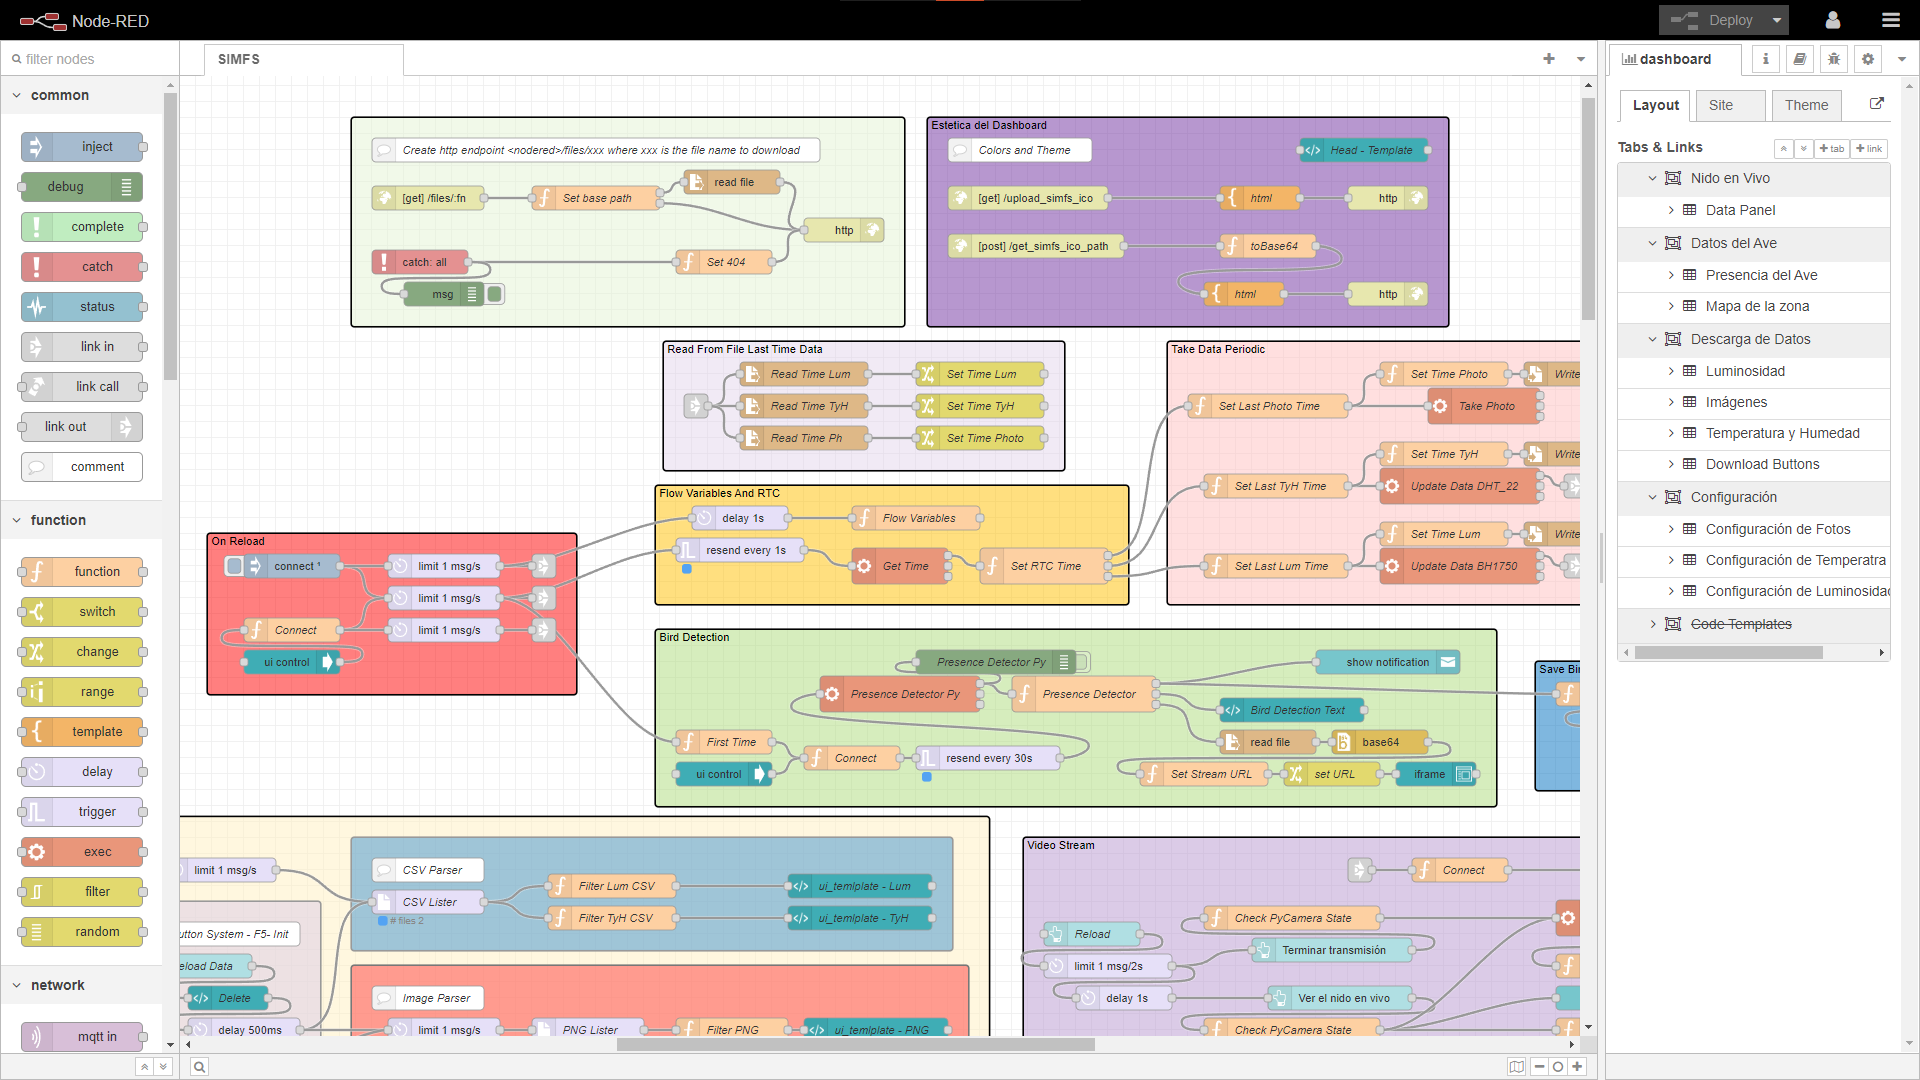
\includegraphics[width=0.9\linewidth]{ImagenesIngenieria de Detalle/Node-Red-Flow}
	\label{fig:node_red_flow}
	\caption{Flujo de nodos del servidor.}
\end{figure}

Dado que este servidor se encuentra corriendo en la R-Pi, al conectarse a la red de esta, se puede acceder a la página mencionada, donde se brindaran varias funcionalidades adicionales a las descargas básicas de los datos requeridos.

La interfaz gráfica a la cual el usuario tiene acceso posee distintas pestañas, donde cada una brinda un parámetro diferente. En la primer pestaña es posible ver las mediciones realizadas de luminosidad, temperatura y humedad en tiempo real. Además como el sistema detecta la presencia del ave, se muestra si este se encuentra dentro del nido o no. Por último se brinda al usuario la posibilidad de ver la una trasmisión en tiempo real del nido por dentro.
\begin{figure}[H]
\centering
    	\minipage{0.49\textwidth}
        	\centering
        	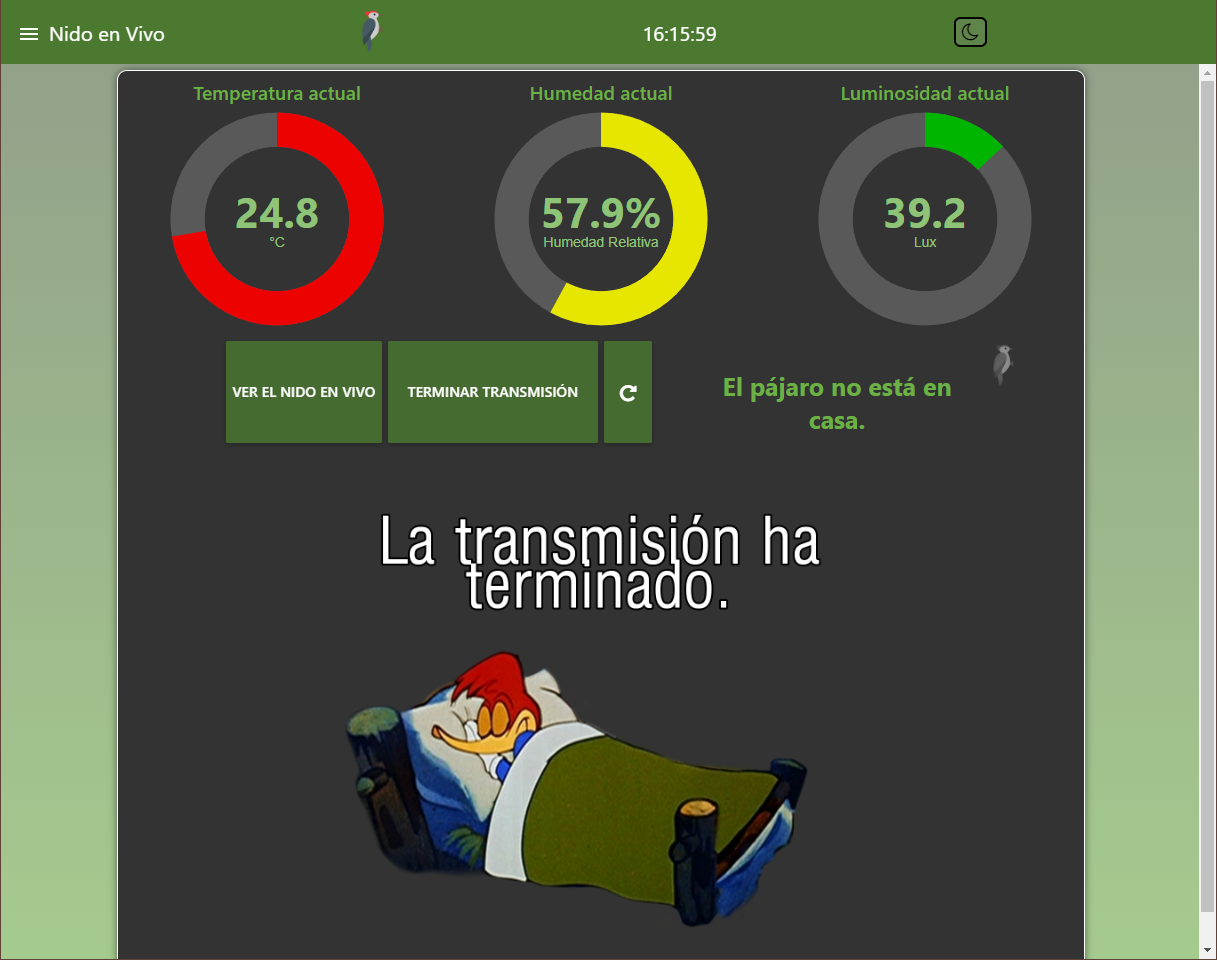
\includegraphics[width=\linewidth]{ImagenesIngenieria de Detalle/Node-Red-Live-Dark}		
			\caption{Interfaz con usuario versión oscura.}
			\label{fig:front_end_dark}
        \endminipage\hfill
        \minipage{0.49\textwidth}
        	\centering
        	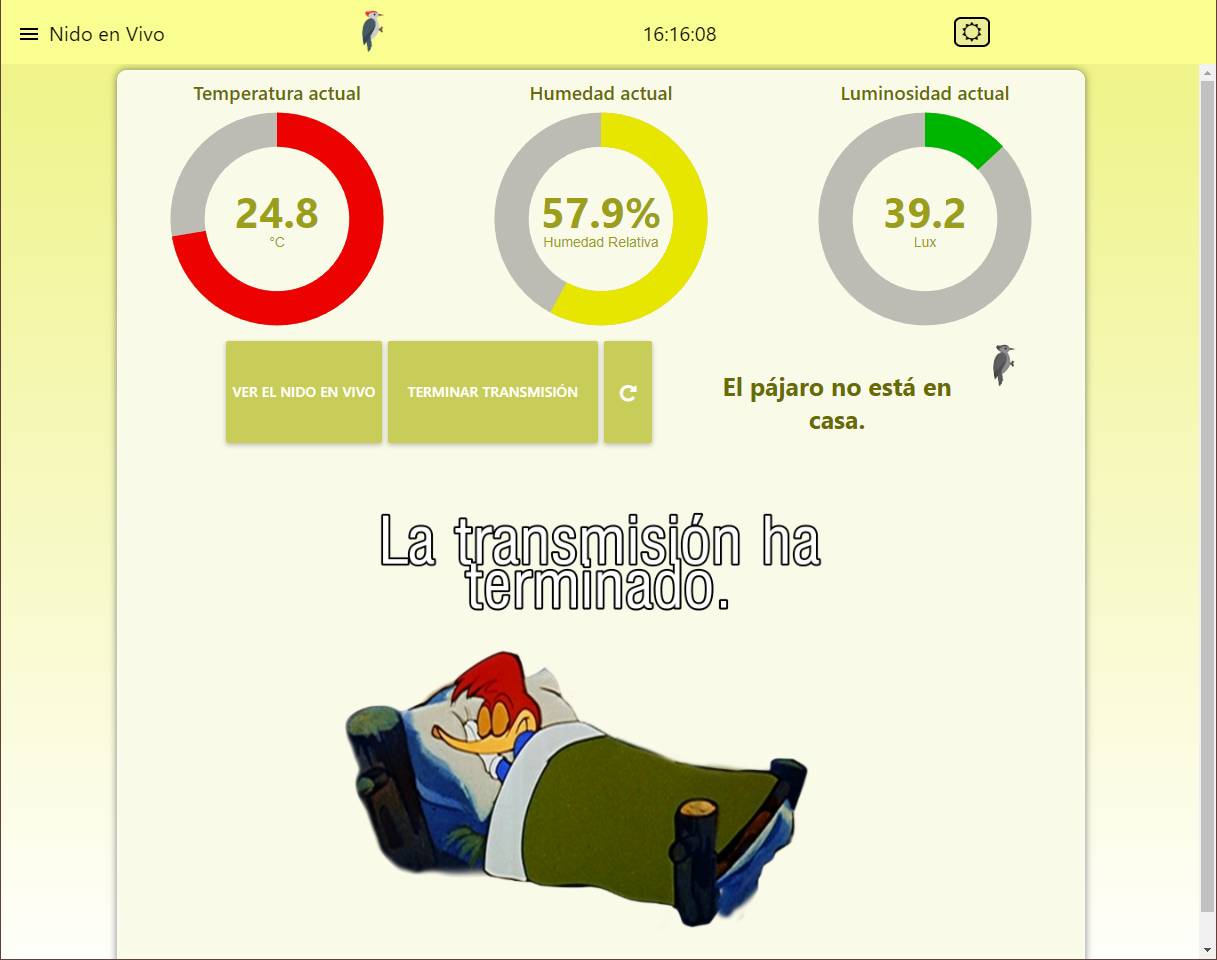
\includegraphics[width=\linewidth]{ImagenesIngenieria de Detalle/Node-Red-Live-Light}				\caption{Interfaz con usuario versión clara.}
			\label{fig:front_end_light}
        \endminipage
	\caption{Página del servidor a la cual accede el usuario.}
	\label{fig:node_red_live}
\end{figure}

En la segunda pestaña, es posible ver datos propios del ave, referidos a su posición. El primero muestra en un gráfico si el ave se ha encontrado dentro o fuera del nido durante un lapso de 24 horas, siendo posible seleccionar el día del cual se quiere ver los datos. Las zonas verdes denotan su estadía en el nido, mientras que las rijas su ausencia. Se muestra también cuanto tiempo duró cada intervalo. El segundo gráfico muestra el recorrido que ha realizado el ave en el entorno del nido en tiempo real.
\begin{figure}[H]
	\centering
    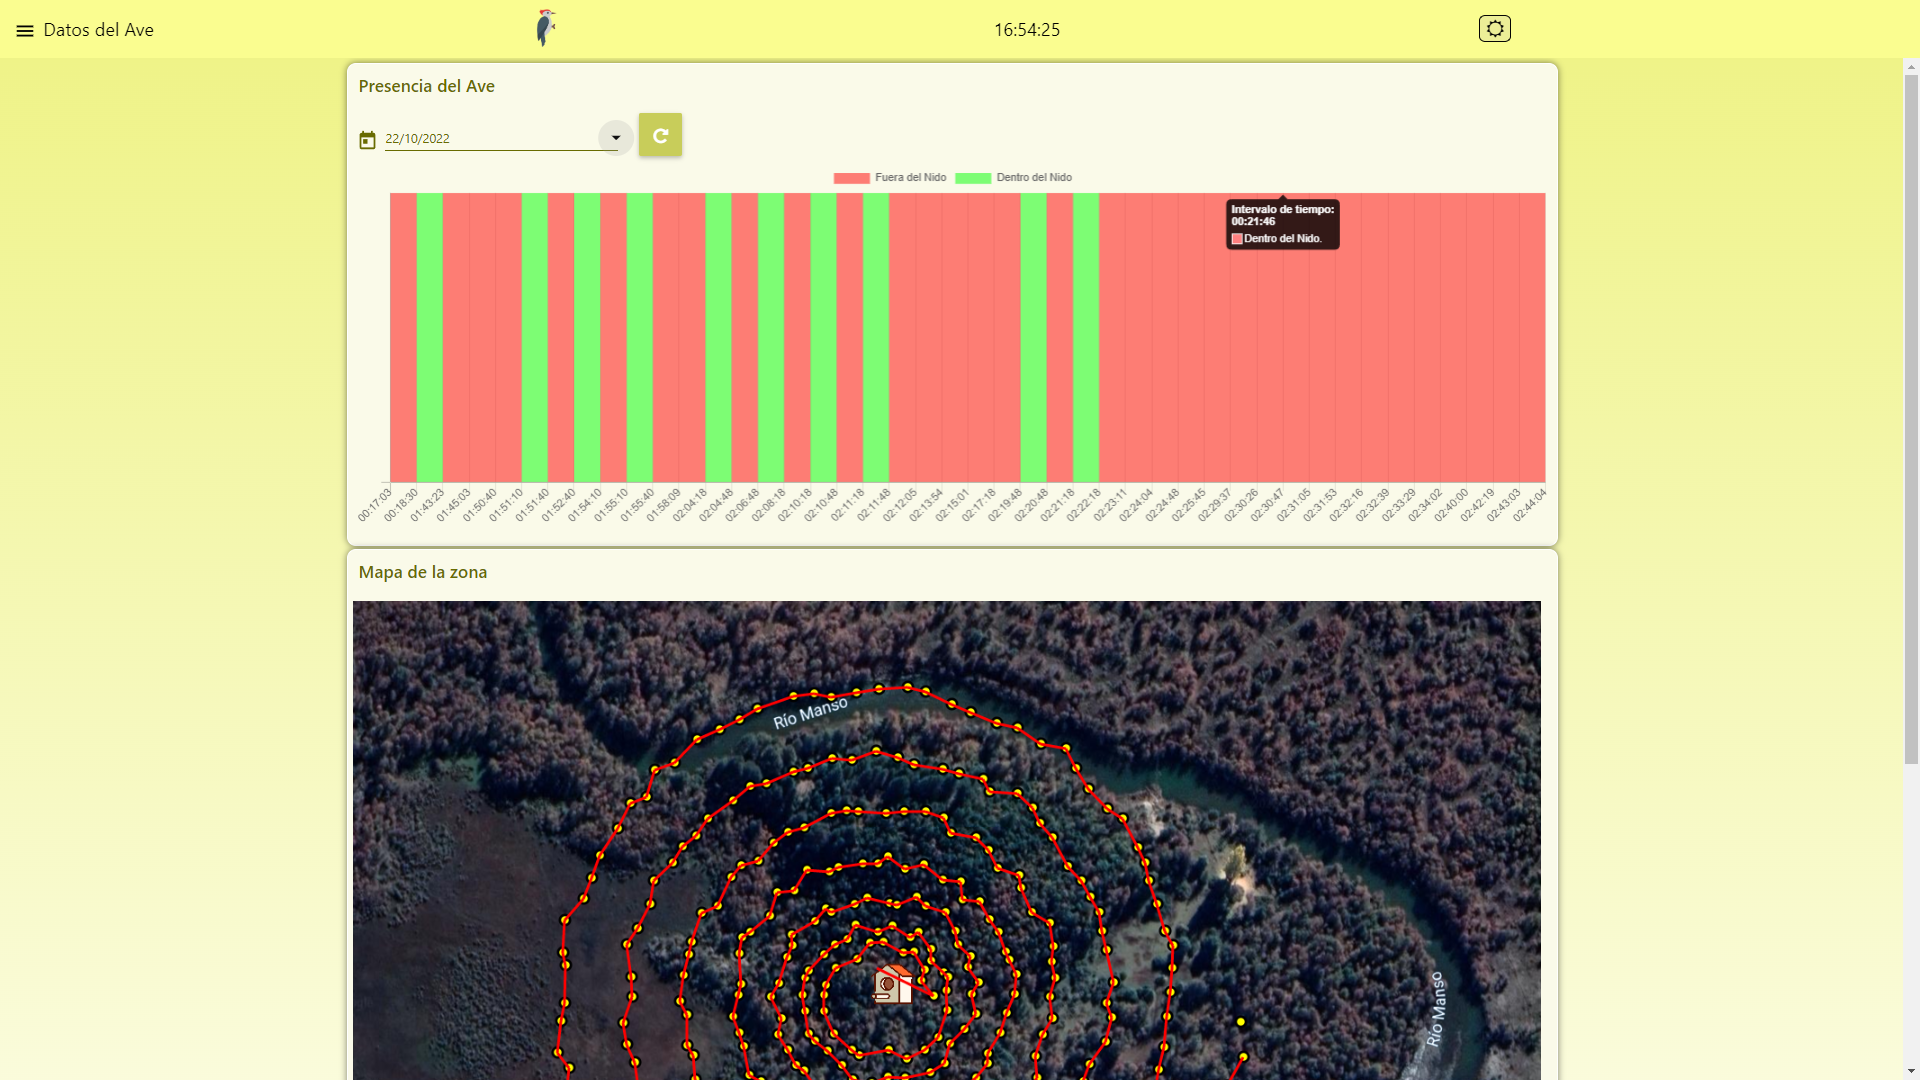
\includegraphics[width=0.7\linewidth]{ImagenesIngenieria de Detalle/Node-Red-Bird-Data}	
	\caption{Datos de presencia y posición del ave.}
	\label{fig:node_red_bird}
\end{figure}

La tercer pestaña es la más importante en cuanto a los requisitos del proyecto. En esta se presentan links de descarga para los datos obtenidos del nido y aquellos provistos por la unidad del pájaro. El usuario puede seleccionar el intervalo de tiempo en el cual desea obtener los datos.

Es posible descargar archivos del formato \quotes{csv} para los datos de luminosidad, temperatura y humedad, \quotes{png} si se desea descargar imágenes de forma individual o \quotes{zip} para el todo el conjunto de fotos mostradas.
\begin{figure}[H]
	\centering
    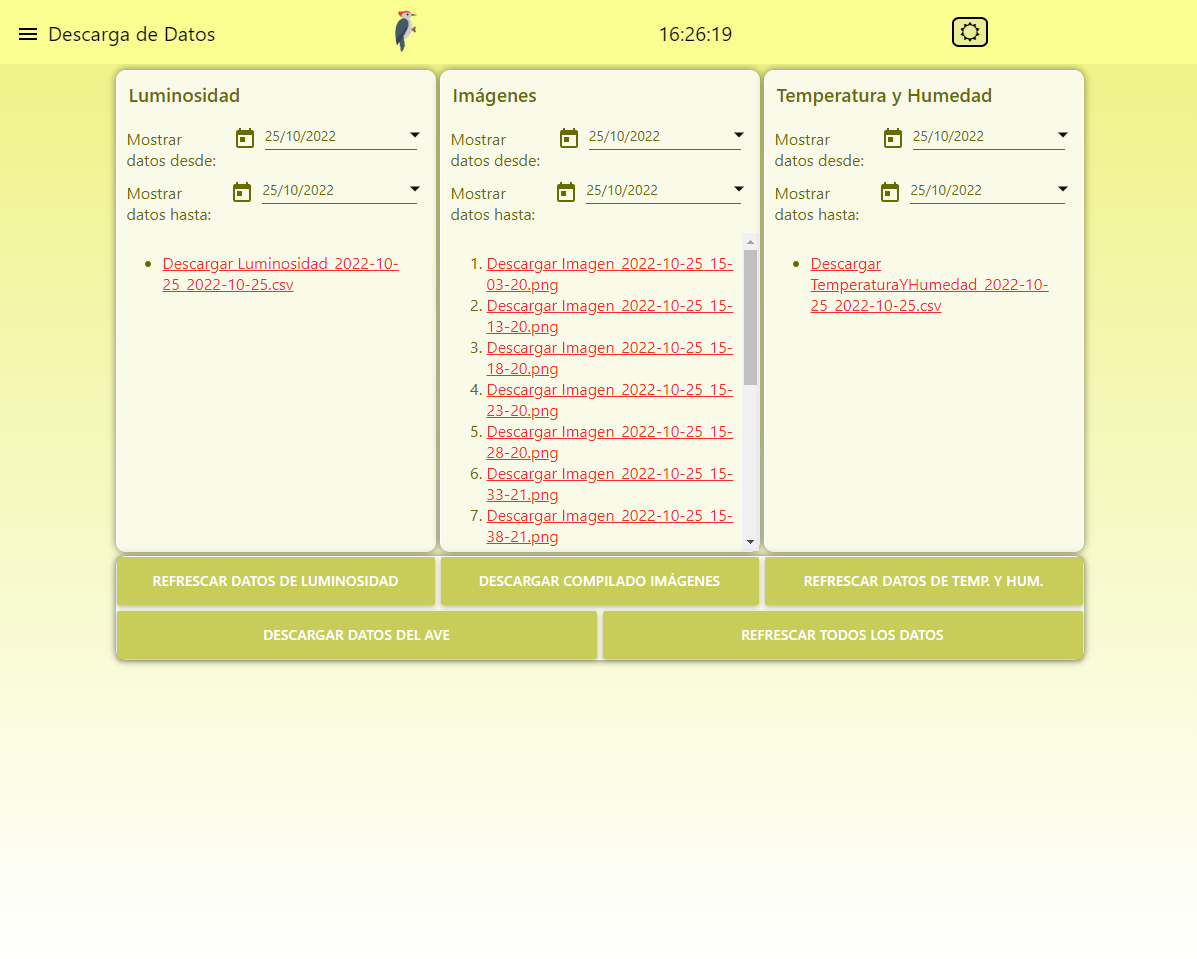
\includegraphics[width=0.7\linewidth]{ImagenesIngenieria de Detalle/Node-Red-Download}	
	\caption{Descarga de datos almacenados.}
	\label{fig:node_red_download}
\end{figure}

La cuarta y última pestaña le brinda al usuario cierto margen de configuración de la toma de datos. Estas opciones le permiten modificar el intervalo de cada medición, es decir cada cuanto tiempo se desea tomar una medición de las variables de interés o cada cuanto se desea tomar una foto.
\begin{figure}[H]
	\centering
    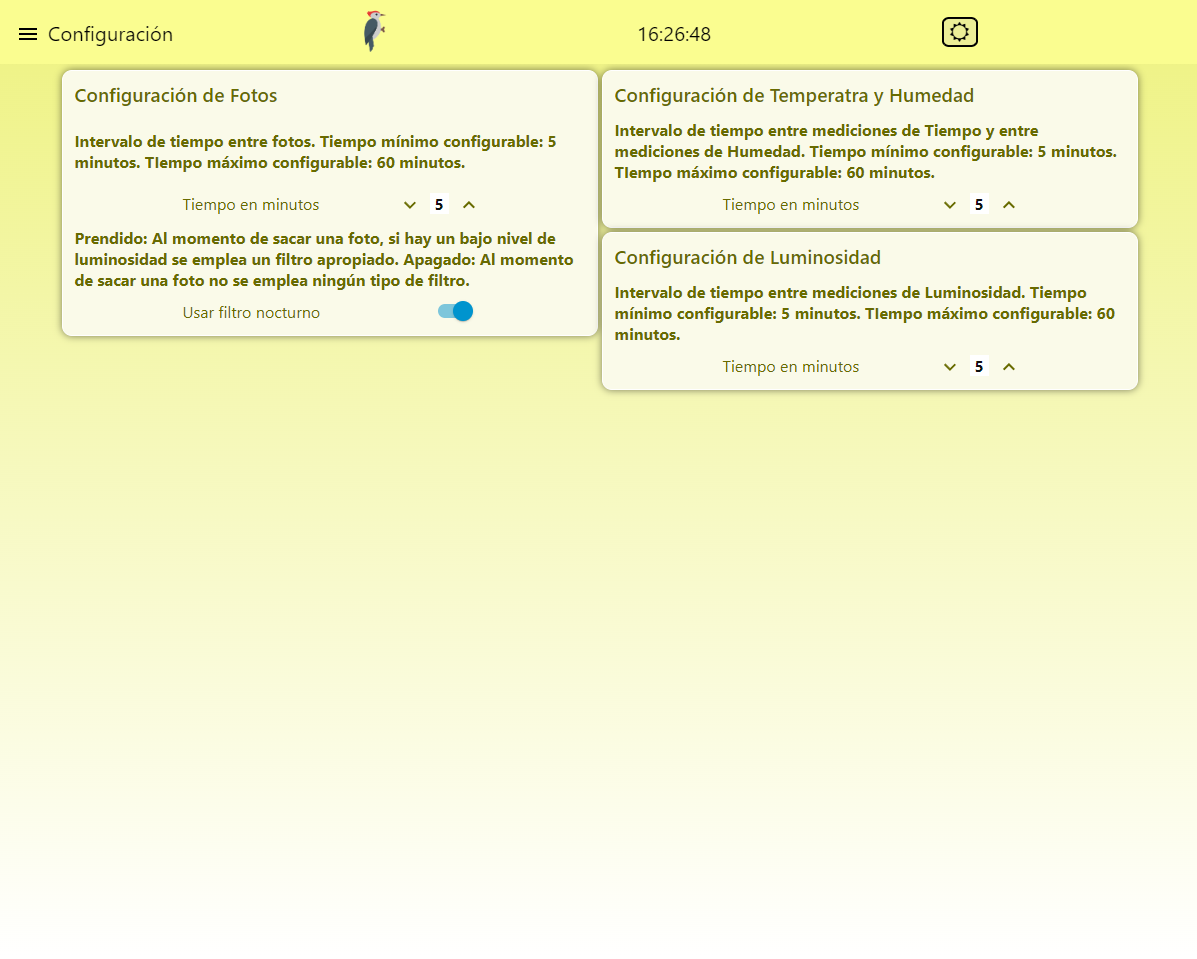
\includegraphics[width=0.7\linewidth]{ImagenesIngenieria de Detalle/Node-Red-Bird-Config}	
	\caption{Configuración de la interfaz gráfica.}
	\label{fig:node_red_config}
\end{figure}

También es posible determinar si se desea o no emplear un filtro en la cámara al momento tomar fotos, considerando el nivel luminosidad. En caso de que dicha variable posea un valor bajo se emplea el filtro mejorando así la luminosidad de la foto.
\begin{figure}[H]
\centering
    	\minipage{0.49\textwidth}
        	\centering
        	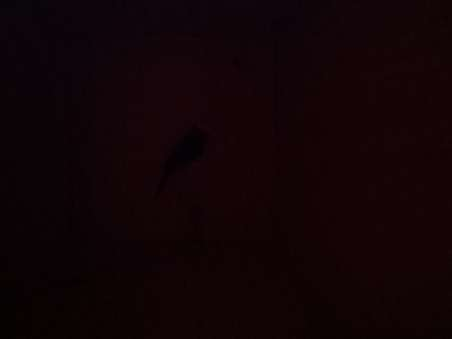
\includegraphics[width=\linewidth]{ImagenesIngenieria de Detalle/ImagenDevSF_2}		
			\caption{Foto tomada sin filtro de luminosidad.}
			\label{fig:foto_camara_sf}
        \endminipage\hfill
        \minipage{0.49\textwidth}
        	\centering
        	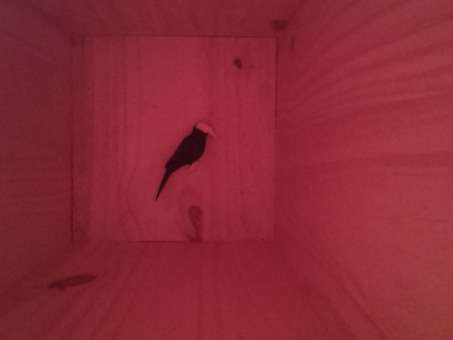
\includegraphics[width=\linewidth]{ImagenesIngenieria de Detalle/ImagenDevCF_2}					\caption{Foto tomada con filtro de luminosidad.}
			\label{fig:foto_camara_cf}
        \endminipage
	\caption{Comparación entre el uso del filtro de luminosidad.}
	\label{fig:foto_camara_filtro}
\end{figure}

Cabe destacar que de la misma forma que se considera un usuario de administrador, la GUI cuenta con una cuenta con contraseña para brindarle acceso al usuario y así evitar el uso de cualquier persona que consiga conexión a la red.